The Table \ref{tab:sdnn_table_blind} presents the standard deviation of the interbeat interval by each participant on each scenes. As it was with the Table \ref{tab:bpm_table_blind}, it is not posible to draw a pattern inside this Table. Different participant had increase, or decrease, with different methods.


\begin{table}[!htb]
\centering
\caption{Average SDNN of the blind participants during the each round and method [ms].}
\label{tab:sdnn_table_blind}
\begin{tabular}{llrrrrr}
\toprule
     &        &    Base &   Audio &  \begin{tabular}[c]{@{}l@{}}Haptic\\ Belt\end{tabular} &  \begin{tabular}[c]{@{}l@{}}Virtual\\ Cane\end{tabular} &  Mixture \\
Participant & Round &         &         &                                                        &                                                         &          \\
\midrule
001C & First &  81.292 & 107.061 &                                                124.737 &                                                 163.968 &  129.054 \\
     & Return & 120.719 & 130.885 &                                                131.590 &                                                 157.589 &  124.786 \\
002C & First &  73.761 &  98.863 &                                                 81.140 &                                                  33.977 &   79.289 \\
     & Return & 108.940 &  49.627 &                                                 42.815 &                                                 114.057 &  107.545 \\
003C & First &  36.870 &  38.325 &                                                 35.101 &                                                  42.392 &   43.692 \\
     & Return &  52.750 &  41.196 &                                                 44.256 &                                                  42.602 &   46.145 \\
004C & First &  70.728 &  86.827 &                                                 62.560 &                                                  85.900 &   70.472 \\
     & Return &  71.950 &  74.895 &                                                 70.017 &                                                  66.089 &  104.040 \\
\bottomrule
\end{tabular}
\end{table}



Inside the barplot Figure \ref{fig:barplot_ecg_sdnn_5_scene_blind} shows the average SDNN in each method. It is posible to notice that some method had an increase and some a decrease in the SDNN. The ones that indicate an increase would mean that the participant felt a lesser mental workload in the "Return" round, whilst the deacrese means the opposite.

\begin{figure}[!htb]
    \centering
    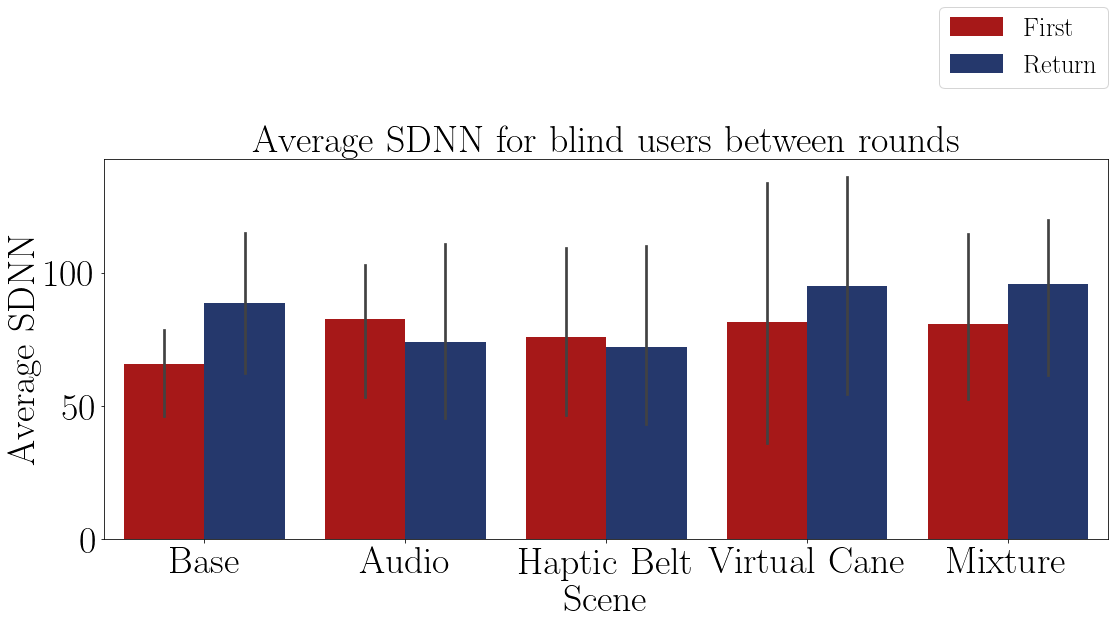
\includegraphics[width = 0.8\linewidth]{Resultados/ECG/Figuras/png/barplot_ecg_sdnn_5_scene_blind.png}
    \caption{Barplot of the average SDNN of the blind participants on each method.}
    \label{fig:barplot_ecg_sdnn_5_scene_blind}
\end{figure}

The Table \ref{tab:sdnn_average_group_blind} presents the average SDNN variation between the rounds. It shows that only the "Audio" and the "Haptic Belt" methods shown a increase in the mental workload.


\begin{table}[!htb]
\centering
\caption{ECG average SDNN for each method of the blind participants.}
\label{tab:sdnn_average_group_blind}
\begin{tabular}{lrrrrr}
\toprule
{} &   Base &  Audio & Haptic Belt & Virtual Cane & Mixture \\
Visual Condition &        &        &             &              &         \\
\midrule
Blind            &  77.13 &  78.46 &       74.03 &        88.32 &   88.13 \\
\bottomrule
\end{tabular}
\end{table}



The Figures \ref{fig:boxplot_ecg_sdnn_blind_scene} presents the distribution of each method SDNN. It noticeable that the "Base" method has a different SDNN than the rest. The "Virtual Cane" also has a different distribution from the rest. The Figure \ref{fig:boxplot_ecg_sdnn_blind_rounds} presents the SDNN grouped by the rounds. It shows a slight difference between the rounds.


\begin{figure}[!htb]
    \centering
    \begin{minipage}{0.45\textwidth}
        \centering
        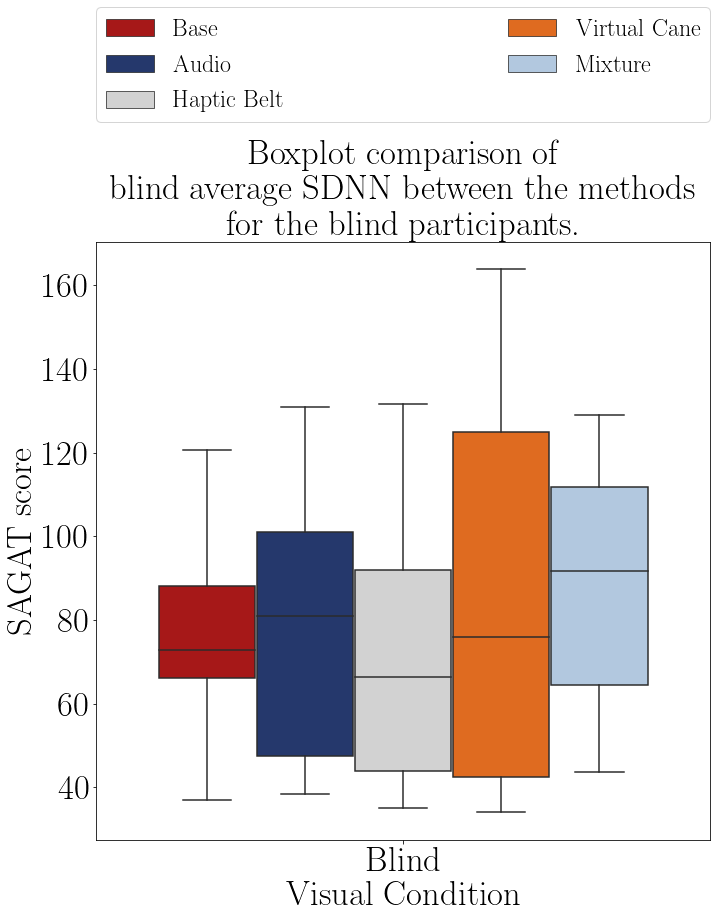
\includegraphics[width = 0.8\linewidth]{Resultados/ECG/Figuras/png/boxplot_ecg_sdnn_blind_scene.png}
        \caption{Boxplot of the SDNN of the blind participants grouped by method.}
        \label{fig:boxplot_ecg_sdnn_blind_scene}
    \end{minipage}
    \begin{minipage}{0.45\textwidth}
        \centering
        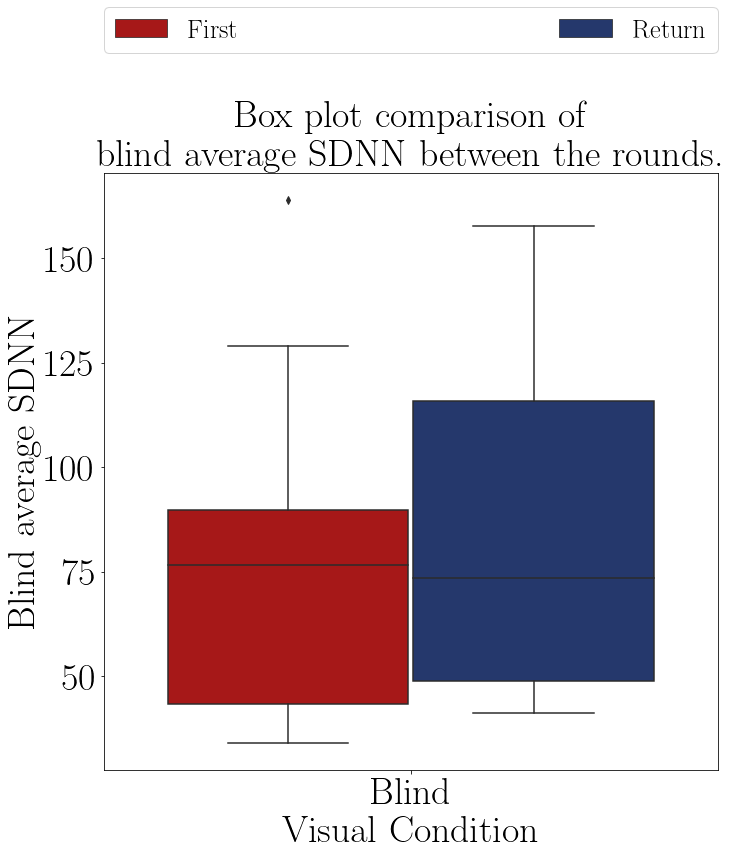
\includegraphics[width = 0.8\linewidth]{Resultados/ECG/Figuras/png/boxplot_ecg_sdnn_blind_rounds.png}
        \caption{Boxplot of the SDNN of the blind participants grouped by round.}
        \label{fig:boxplot_ecg_sdnn_blind_rounds}
    \end{minipage}
\end{figure}

The Figures \ref{fig:qqplot_sdnn_two_way_blind} and \ref{fig:residplot_sdnn_two_way_blind} shows the distribution and variance of the Table \ref{tab:sdnn_table_blind}. These Figures shows that the data are normally distributed but the participants had different  that the methods have a similar variance.
The Table \ref{tab:blocdanova_sdnn_two_way_blind} shows the ANOVA test p-value of the heartbeat interval variance of the “blind” sample. The p-value indicates that there is no effect of any factor.


\begin{table}[!htb]
\centering
\caption{Anova p-value for the average SDNN on each method for blinded users.}
\label{tab:blocdanova_sdnn_two_way_blind}
\begin{tabular}{lrrrrr}
\toprule
          Source & P-Value \\
\midrule
    \    Methods &   0.486 \\
     \    Rounds &   0.223 \\
\    Interaction &   0.473 \\
\bottomrule
\end{tabular}
\end{table}



\begin{figure}[!htb]
    \centering
    \begin{minipage}{0.45\textwidth}
        \centering
        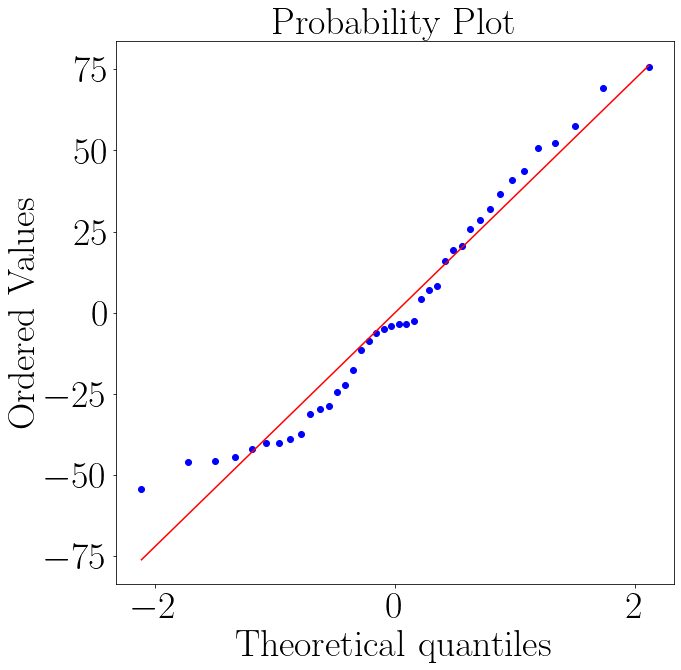
\includegraphics[width = 0.8\linewidth]{Resultados/ECG/Figuras/png/qqplot_sdnn_two_way_blind.png}
        \caption{QQ plot of the SDNN of the blind participants on each method.}
        \label{fig:qqplot_sdnn_two_way_blind}
    \end{minipage}
    \begin{minipage}{0.45\textwidth}
        \centering
        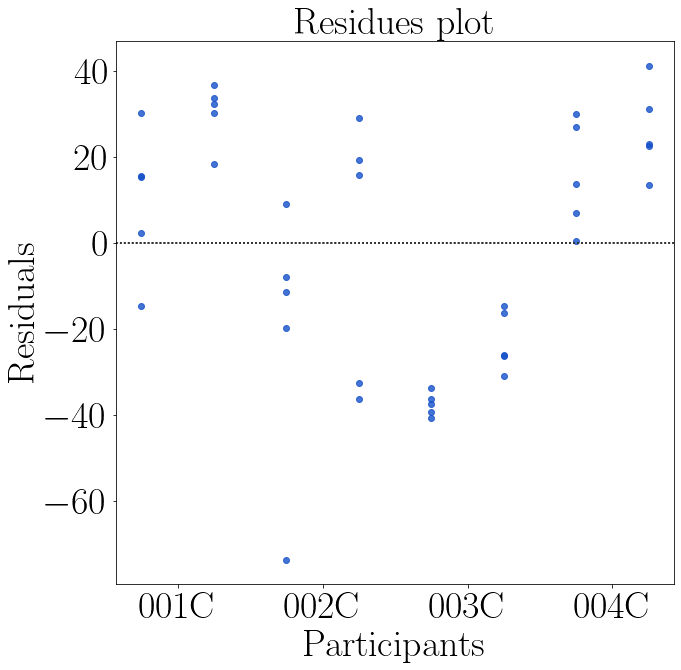
\includegraphics[width = 0.8\linewidth]{Resultados/ECG/Figuras/png/residplot_sdnn_two_way_blind.png}
        \caption{Residual plot of the SDNN of the blind participants on each method.}
        \label{fig:residplot_sdnn_two_way_blind}
    \end{minipage}
\end{figure}

%
\begin{table}[!htb]
\centering
\caption{Cross validation p-value for the average SDNN on each method for blinded users.}
\label{tab:lsd_sdnn_two_way}
\begin{tabular}{rclr}
\toprule
      \multicolumn{3}{c}{Method} &                                           Analysis \\
\midrule
              Base & $X$ & Audio &                   $H_0 : \mu_{Base} = \mu_{Audio}$ \\
        Base & $X$ & Haptic Belt &             $H_0 : \mu_{Base} = \mu_{Haptic Belt}$ \\
       Base & $X$ & Virtual Cane &        $H_1 : \mu_{Base} \ne \mu_{Virtual Cane}**$ \\
            Base & $X$ & Mixture &             $H_1 : \mu_{Base} \ne \mu_{Mixture}**$ \\
       Audio & $X$ & Haptic Belt &        $H_1 : \mu_{Audio} \ne \mu_{Haptic Belt}**$ \\
      Audio & $X$ & Virtual Cane &       $H_1 : \mu_{Audio} \ne \mu_{Virtual Cane}**$ \\
           Audio & $X$ & Mixture &            $H_1 : \mu_{Audio} \ne \mu_{Mixture}**$ \\
Haptic Belt & $X$ & Virtual Cane & $H_1 : \mu_{Haptic Belt} \ne \mu_{Virtual Cane}**$ \\
     Haptic Belt & $X$ & Mixture &      $H_1 : \mu_{Haptic Belt} \ne \mu_{Mixture}**$ \\
    Virtual Cane & $X$ & Mixture &         $H_0 : \mu_{Virtual Cane} = \mu_{Mixture}$ \\
\bottomrule
\end{tabular}
\end{table}



The Table \ref{tab:blocdanova_sdnn_two_way_blind} does not prove that any method or round has some influence in the heartbeat interval variance, thus in the Mental Workload. Although, in the Figure \ref{fig:boxplot_ecg_sdnn_blind_scene} it is posible to notice that the "Base" method has a different distribution. As it has already commented before, maybe the result of the anova test is a conseguence of a small sample size.

\FloatBarrier